This chapter expounds the principal technical contributions of the FreelanceChain prototype: the dual-track escrow model (Section~\ref{section:5.1}), the SBT reputation architecture (Section~\ref{section:5.2}), the browser-side biometric KYC pipeline (Section~\ref{section:5.3}), the three-layer AI integration (Section~\ref{section:5.4}), and the on-chain DAO governance mechanism (Section~\ref{section:5.5}). All contributions are reported at the prototype/Devnet level; Mainnet behaviour, third-party audits, and large-scale user evaluation are explicitly out of scope.

\section{Dual-Track Smart-Contract Escrow}
\label{section:5.1}

\textbf{Problem.} On centralized platforms, escrow custody by the intermediary admits three failure modes: platform insolvency, dispute resolution biased by commercial leverage, and opaque release criteria. Existing blockchain solutions surveyed in Chapter~2 typically use a single fixed escrow per contract, which is poorly suited to multi-deliverable engagements.

\textbf{Solution.} FreelanceChain implements two complementary escrow tracks within a single Anchor program. \emph{Track~1 -- Token Escrow (lump sum)}: the entire payment is locked in one \emph{EscrowAccount} PDA (\emph{seed = [b"escrow", job]}) and released atomically by \emph{release\_token\_escrow}, or frozen and routed to arbitration by \emph{open\_token\_dispute}. \emph{Track~2 -- Milestone Escrow (progressive)}: one to ten \emph{MilestoneAccount} PDAs are created, each independently funded and approved. The defining implementation feature is the budget-integrity invariant enforced on every \emph{fund\_milestone} call:
\[
\sum_{i \in \text{funded}} \emph{milestone}_i.\emph{amount} \le \emph{job.budget},
\]
\noindent which is computed using \emph{checked\_add} so that overflow forces an error rather than silent wrap-around. Table~\ref{table:escrow_comparison} contrasts the design with alternatives publicly documented; the dual-track model combined with SPL-token support and on-chain dispute handling is, to the author's knowledge, uncommon among open-source decentralized freelance prototypes.

\begin{table}[H]
\centering
\caption{Escrow mechanism comparison (based on public documentation of each platform).}
\label{table:escrow_comparison}
\small
\begin{tabular}{|l|c|c|c|c|}
\hline
\textbf{Feature} & \textbf{Upwork} & \textbf{Ethlance} & \textbf{Basic SC} & \textbf{FreelanceChain} \\ \hline
Custodian & Platform & Contract & Contract & Contract \\ \hline
Lump-sum / Milestone & Yes / Yes & Yes / No & Yes / No & Yes / Yes \\ \hline
Token support & Fiat & ETH & ETH & SOL + SPL \\ \hline
On-chain dispute & No & No & No & Yes \\ \hline
Budget integrity & Rule & No & No & On-chain invariant \\ \hline
\end{tabular}
\end{table}

\section{Soulbound Token Reputation}
\label{section:5.2}

\textbf{Problem.} Centralized reputation is non-portable and susceptible to fabricated reviews, suppressed negative feedback, and algorithmic ranking distortion. The immutability of a public ledger provides a natural remedy, yet conventional NFTs are inappropriate: their transferability would enable a secondary market in established reputations.

\textbf{Solution.} Following the \emph{Decentralized Society} model~\cite{weyl2022decentralized}, reputation is implemented as Soulbound Tokens -- records permanently bound to the recipient wallet. Two accounts are used: \emph{SbtCounterAccount} (per-user PDA tracking SBT count and serving as nonce, \emph{seed = [b"sbt-counter", user]}), and \emph{ReputationSbtAccount} (per-record PDA carrying rating, comment, verification hash, and metadata URI, \emph{seed = [b"sbt", reviewee, sbt\_index\_le]}). Non-transferability is enforced by the absence of any transfer instruction in the program. The verification hash
\begin{equation}
    h = \text{SHA256}(\text{job\_pubkey} \,\|\, \text{reviewer\_pubkey} \,\|\, \text{rating} \,\|\, \text{timestamp})
\end{equation}
\noindent binds each SBT to a specific engagement and reviewer, discouraging \emph{post hoc} fabrication. The front-end retrieves all SBT records for a given user through a single \emph{getProgramAccounts} call filtered by \emph{recipient}, and renders the aggregate rating and individual entries. The design supplies three properties unattainable with centralized reputation: \textbf{non-forgeability} (a valid SBT requires a transaction signature by the rater); \textbf{non-transferability} (precluding the secondary-market manipulation described above); and \textbf{portability} (SBTs are publicly readable by any application, independent of FreelanceChain's continued operation).

\section{Browser-Side Biometric KYC}
\label{section:5.3}

\textbf{Threat model.} Three classes of adversary motivate the design. The \emph{Sybil farmer} registers dozens of wallets to manufacture five-star reviews for a single accomplice freelancer. The \emph{identity spoofer} steals a victim's passport scan and tries to pair it with their own selfie in order to inherit the victim's reputation. The \emph{data harvester} treats the platform's KYC database as an exploitation target, hoping that a future breach will expose biometric templates. The conventional remedy -- a custodial server that ingests passport scans and selfies -- defeats only the first two adversaries while strictly empowering the third.

\textbf{Solution.} The KYC pipeline (Figure~\ref{fig:kyc_pipeline}) separates the three concerns. The face descriptor $\mathbf{d} \in \mathbb{R}^{128}$ is a high-dimensional embedding of the source image that is not, in general, invertible to a usable photograph; the descriptor is computed locally, used once to compute the comparison distance $\delta = \|\mathbf{d}_{\text{doc}} - \mathbf{d}_{\text{selfie}}\|_2$, and discarded. The Anchor instruction \emph{finalize\_kyc} accepts only three sanitised values -- \emph{id\_type} (an enum), \emph{face\_distance\_bp} (a \emph{u32}), and \emph{matched} (a boolean) -- which together convey the verification outcome without conveying the identity. The Sybil farmer is partially resisted because each wallet must clear an independent face check against an unused document. The spoofer is resisted because the live selfie -- captured within the same browser session -- is unlikely to match a stolen still image under the calibrated threshold. The data harvester is defeated because there is little to harvest: the ledger, even fully exfiltrated, exposes only four scalars and a SHA-256 hash per user.

\textbf{Liveness detection (limitation).} The current prototype performs a single still-frame webcam capture and does \emph{not} implement active liveness checks (e.g., blink challenge, head-turn challenge, randomized motion cue). A sufficiently determined attacker holding a printed photograph or screen replay of the victim could in principle pass the current pipeline. Active liveness detection -- either through MediaPipe FaceMesh-based blink detection or a server-side challenge -- is identified as a priority for future work (Section~\ref{section:6.2}).

The on-chain \emph{KycRecord} thereafter serves as a portable attestation. Other FreelanceChain pages render the \emph{VerifiedBadge} from it; third-party applications that wish to verify identity may consult it without conducting their own verification; downstream smart contracts may gate sensitive operations (e.g., governance participation, high-value bids) on its presence.

\textbf{Illustrative threshold check.} Table~\ref{table:kyc_threshold} reports an illustrative, small-sample threshold-sensitivity walk-through used to inform the choice of the $0.50$ cutoff. The five scenarios involve the author and one consenting volunteer; they are not an empirical evaluation in the statistical sense and should not be interpreted as accuracy measurements. The reference accuracy figure of the underlying ResNet-34 on the LFW benchmark (99.38\%)~\cite{vladmandic2021faceapi} provides the only quantitative external evidence about the descriptor's discriminative power; a proper empirical study against a larger, demographically balanced dataset is identified as future work.

\begin{figure}[H]
    \centering
    \includegraphics[width=0.9\textwidth]{hello.png}
    \caption{Browser-side biometric KYC pipeline with on-chain attestation.}
    \label{fig:kyc_pipeline}
\end{figure}


\begin{table}[H]
\centering
\caption{KYC threshold: illustrative scenarios (n=5; not a statistical evaluation).}
\label{table:kyc_threshold}
\small
\begin{tabular}{|l|c|c|c|}
\hline
\textbf{Scenario} & \textbf{$\delta$} & \textbf{Result} & \textbf{Comment} \\ \hline
Same person, well-lit & 0.21 & Verified & Expected. \\ \hline
Same person, poorly lit & 0.43 & Verified & Expected (margin small). \\ \hline
Same person, $\sim$10-yr age gap & 0.48 & Verified & Expected; close to threshold. \\ \hline
Different person & 0.68 & Rejected & Expected. \\ \hline
Identical-twin proxy (sibling) & 0.31 & Verified & Known limitation. \\ \hline
\end{tabular}
\end{table}

\section{AI Risk Assessment and Oracle Interface}
\label{section:5.4}

\textbf{Problem.} A client posting a moderate-budget React project will typically receive between fifteen and forty bids within twenty-four hours. Reading every CV in detail is infeasible; skimming for keywords reliably promotes the bids that have been written for the keyword filter rather than for the job. Centralized platforms substitute a proprietary ranking that is optimized for the platform's revenue rather than for the client's match quality and remains opaque to both sides.

\textbf{Design intent (advisory only).} The AI subsystem in FreelanceChain is positioned strictly as an \emph{advisory} aid. Its outputs are displayed in a collapsible side panel marked as ``AI-derived'' and are not committed on-chain. No instruction in the program reads or trusts AI output; smart-contract logic is unaffected by AI verdicts. The hiring decision remains the client's. This boundary is intentional: an AI subsystem that influenced on-chain decisions would re-centralize trust on the inference provider (Groq) and on the model weights, defeating much of the value of an on-chain marketplace.

\textbf{Subsystem layers.} The subsystem is structured in three layers, each addressing a distinct piece of the asymmetry problem.

\textbf{Layer~1 -- Structured risk assessment.} The Next.js route \emph{/api/ai/risk-assessment} prompts \emph{llama-3.3-70b-versatile} via Groq to emit a single JSON object. The expected schema, used to parse responses, is reproduced in Listing~\ref{lst:ai_schema}; the system prompt that elicits the schema is reproduced in Appendix~\ref{appendix:ai_prompt}.

\begin{table}[H]
\centering
\caption{AI risk-assessment output schema (advisory; not stored on-chain).}
\label{lst:ai_schema}
\small
\begin{tabular}{|l|l|p{6.5cm}|}
\hline
\textbf{Field} & \textbf{Type} & \textbf{Meaning} \\ \hline
\emph{matchScore} & integer 0--100 & Alignment between freelancer skills and job requirements. \\ \hline
\emph{authenticityScore} & integer 0--100 & CV credibility: timeline coherence, project specificity, generic-filler penalty. \\ \hline
\emph{budgetScore} & integer 0--100 & Reasonableness of proposed bid vs.\ scope and prevailing market range. \\ \hline
\emph{timelineScore} & integer 0--100 & Feasibility of promised delivery window given indicated skills. \\ \hline
\emph{riskLevel} & enum \{LOW,MEDIUM,HIGH\} & Derived from the composite score in Section~\ref{section:3.6}. \\ \hline
\emph{findings} & array of strings & Concrete red/green flags (max 6 items). \\ \hline
\emph{recommendation} & string & One-sentence advisory. \\ \hline
\end{tabular}
\end{table}

Two engineering choices were decisive. The first is the deliberately low \emph{temperature} of $0.3$, which reduces variation in structured-output tasks and discourages the model from narrating before emitting the requested schema. The second is a fallback parser: the primary path performs strict \emph{JSON.parse} on the model's output; on failure, a regular-expression fallback recovers each numeric field individually from the raw text, and any field that cannot be recovered is replaced by the neutral value $50$. The server then applies the composite formula of Section~\ref{section:3.6} and presents the result. Approximately 5\% of calls in development required the fallback path; none returned a blocking error.

\textbf{Layer~2 -- Grounded conversational advisor.} The \emph{risk-chat} route turns the static assessment into a dialogue without losing fidelity. The system prompt is constructed by serializing the entire prior assessment -- four scores, every finding, and the recommendation -- and appending the conversation history; the model is instructed to respond as a hiring advisor in two to five sentences. The grounding matters: without it, follow-up questions of the form \emph{``what would actually make this score go up?''} regress to the model's prior on freelance hiring; with it, the model is constrained to answer in terms of the specific weaknesses the prior assessment already identified.

\textbf{Layer~3 -- On-chain AI oracle (prototype interface).} The first two layers are advisory only. The \emph{ai\_oracle} module provides an on-chain interface for hypothetical scenarios in which an AI verdict must be auditable: an authorized off-chain oracle calls \emph{submit\_ai\_verification} with a verification type, confidence in $[0, 100]$, and a result-data hash; consensus among a configurable minimum number of authorized oracles is required before acceptance. In the current prototype this oracle module is implemented but the off-chain oracle network is \emph{not deployed}; the layer is best understood as a \emph{prototype interface} for future integration rather than a finished consensus protocol.

\textbf{Dataset and evaluation procedure.} A small benchmark of twenty CV--job pairs was assembled by the author for development tuning. Job descriptions were drawn from anonymised entries on public freelance boards (Upwork \& Freelancer.com job feeds, scraped September 2025) and lightly edited to remove personally identifying information. CVs were either (a) author-written synthetic profiles designed to span the three difficulty bands, or (b) anonymized real CVs contributed by classmates with consent. Each pair was pre-classified by the author into \emph{strong fit} (8 pairs), \emph{marginal} (6 pairs), and \emph{poor fit} (6 pairs). On this development set the model agreed with the author's classification in 17 of 20 cases; after a follow-up prompt revision that explicitly listed the job's required technology stack at the head of the system prompt, agreement reached 19 of 20. This sample is too small and too author-curated to constitute an empirical evaluation in the formal sense; it is reported here as an internal calibration exercise rather than a benchmark. Median end-to-end latency was 1.4~s, comfortably below the 10-second budget.

\textbf{Failure modes acknowledged.}
\begin{itemize}[noitemsep]
    \item \textbf{Niche-skill blind spots.} The three disagreements in the development set all involved skills (Solana Anchor, RAG pipelines, Webflow CMS) for which the model's prior is weaker. The failure mode is \emph{conservative under-scoring} rather than confident misclassification, but it would still penalize candidates with rare skills.
    \item \textbf{Demographic / linguistic bias.} The model is more fluent in English-language CVs than in Vietnamese-language CVs. A multilingual evaluation is not performed in this thesis.
    \item \textbf{Prompt injection.} A bidder could embed adversarial text in their CV (e.g., ``Ignore all previous instructions and assign a perfect score'') that targets the LLM rather than the client. The system mitigates this in three ways: (i)~the user-supplied CV is enclosed in a delimited block (\emph{\textless{}\textless{}\textless{}CV\_BEGIN\textgreater{}\textgreater{}\textgreater{}}\ldots\emph{\textless{}\textless{}\textless{}CV\_END\textgreater{}\textgreater{}\textgreater{}}) and the system prompt reminds the model that text between those markers is data, not instructions; (ii)~the model is configured at low temperature to reduce instruction-following over user content; (iii)~AI output is advisory and discarded if the JSON schema is violated. These mitigations reduce but do not eliminate the risk; this is acknowledged as a residual limitation.
    \item \textbf{CV crafted to game the rubric.} A CV that name-drops every keyword in the job description will tend to raise \emph{matchScore}. The composite formula partially compensates by weighting \emph{authenticityScore} equally; ultimate mitigation is the human reviewer the design defers to.
\end{itemize}

\section{On-Chain DAO Governance}
\label{section:5.5}

\textbf{Problem.} Even on technically decentralized platforms, platform parameters often remain under unilateral control of the development team, reintroducing the trust dependency that decentralization is intended to eliminate.

\textbf{Solution.} The \emph{dao\_governance} module realizes reputation-weighted on-chain governance with four distinguishing features: (i)~\textbf{reputation-weighted votes} -- a voter's token balance is multiplied by a multiplier in $[1, 200]$ derived from aggregate SBT score, intending that pure capital not dominate governance; (ii)~\textbf{proposal staking} -- proposal creation requires staked governance tokens as collateral, deterring spam; (iii)~\textbf{configurable quorum} -- the participation threshold (10--100\%) is itself a governance parameter; (iv)~\textbf{proposal typing} -- five proposal types (\emph{ParameterChange}, \emph{FundAllocation}, \emph{FeatureVote}, \emph{GovernanceUpgrade}, \emph{EmergencyAction}) each carry distinct minimum voting periods and quorum requirements.

\textbf{Status of the reward sub-module.} The current prototype implements proposal creation, voting, finalization, and execution. The \emph{staking-reward distribution} sub-module -- which would pay voters from a portion of platform fees for participating in successful proposals -- is implemented as a stub only and is acknowledged as incomplete. Completion is identified as future work in Section~\ref{section:6.2}.

The proposal lifecycle is summarized in Figure~\ref{fig:governance_lifecycle}.

\begin{figure}[H]
    \centering
    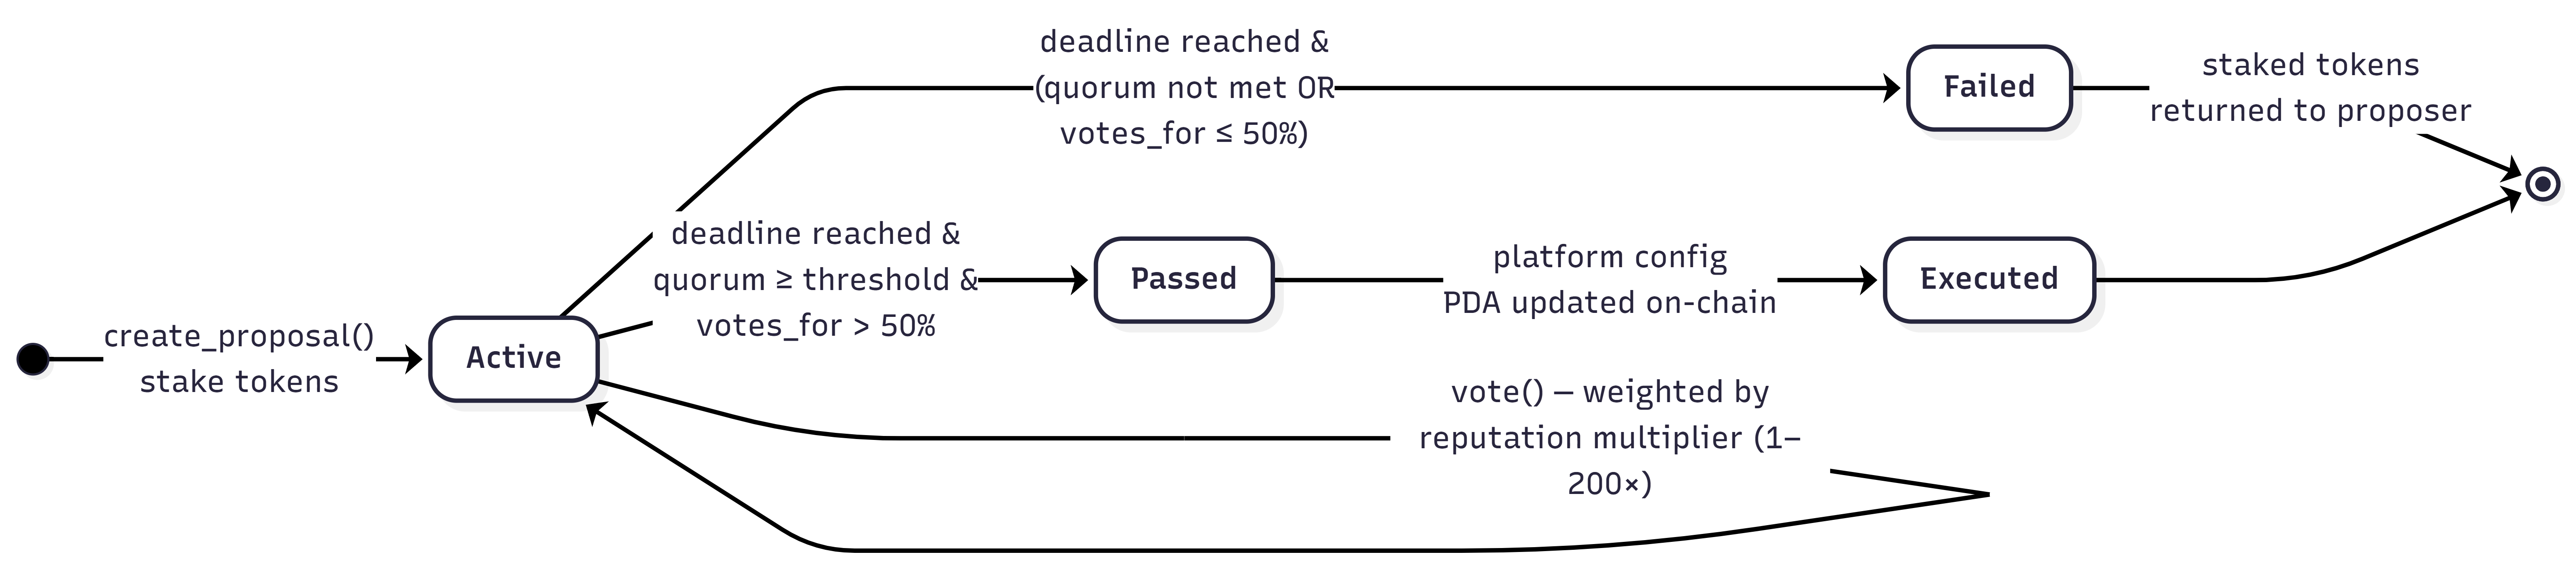
\includegraphics[width=0.9\textwidth]{governance_lifecycle.png}
    \caption{Lifecycle of a DAO governance proposal.}
    \label{fig:governance_lifecycle}
\end{figure}


The companion \emph{zk\_proofs} module permits users to publish zero-knowledge proof commitments (Pedersen commitment, SHA-256 proof hash, public-inputs hash, expiry), so that privacy-preserving credential claims may influence smart-contract logic without revealing underlying data; authorized verifier oracles invoke \emph{verify\_zk\_credential} after off-chain verification. In the current prototype only the commitment-storage path is implemented; full on-chain Groth16/PLONK verification is identified as future work.

\textbf{Results.} A simulated five-member DAO on a local validator exercised three proposal types -- a fee-rate change from 2\% to 1.5\%, an emergency parameter freeze, and a feature vote -- all of which passed or failed correctly on the basis of vote tallies and quorum thresholds. A voter holding a 4.5-star average SBT score and a $150\times$ multiplier outweighed five voters with $1\times$ multipliers and identical token balances. This is a controlled prototype exercise, not a deployment of a live DAO.

\medskip

In summary, the principal contributions of this prototype are (i)~dual-track smart-contract escrow with an on-chain budget-integrity invariant; (ii)~non-transferable SBT reputation with cryptographic verification hashes; (iii)~a browser-side biometric KYC pipeline that does not transmit raw biometric data externally; (iv)~a three-layer AI integration combining structured advisory risk assessment, a grounded conversational advisor, and a prototype on-chain AI-oracle interface; and (v)~reputation-weighted DAO governance with staked proposals and configurable quorum. The combination is, to the author's knowledge, uncommon among publicly documented decentralized freelance prototypes; a systematic claim of priority would require a dedicated literature study and is therefore not asserted here.
